\documentclass{beamer}

% Minimal theme
\usetheme{default}

% Remove navigation symbols
\setbeamertemplate{navigation symbols}{}
\setbeamertemplate{footline}{}

% Package for including PDF pages
\usepackage{pdfpages}

% Additional packages for plots
\usepackage{pgfplots}
\usepackage{tikz}
\pgfplotsset{compat=1.18}

% Define link color
\definecolor{linkblue}{RGB}{0,128,128}
\hypersetup{urlcolor=linkblue, colorlinks=true, linkcolor=linkblue, citecolor=linkblue}

\title{Gradient Descent - Step Size}
\author{ }
\date{ }

\begin{document}

\begin{frame}
   	\titlepage
\end{frame}


\section{Direction + Step Size}



\includepdf[pages={1-11}, scale=1.35, offset=2.5cm -0.5cm]{slides_lmu/04_first_order.pdf}


\section{Line Search Methods}
\begin{frame}
	\centering
	\Huge Line Search Methods

\end{frame}

\begin{frame}{Videos}
	
\begin{itemize}
    \item \href{https://www.youtube.com/watch?v=MzmqM0tuO1Q&list=PL10NOnsbP5Q7wNrYItE2GhKq05cVov97e&index=4}{\textcolor{linkblue}{Inexact Line Search}}
    
    \item \href{https://www.youtube.com/watch?v=X4Pjd-1R-jI&list=PL10NOnsbP5Q7wNrYItE2GhKq05cVov97e&index=6}{\textcolor{linkblue}{Armijo Condition}}
    
    \item \href{https://www.youtube.com/watch?v=5upFcYJqSwo&list=PL10NOnsbP5Q7wNrYItE2GhKq05cVov97e&index=7}{\textcolor{linkblue}{Wolfe 2nd Condition}}
    
    \item \href{https://www.youtube.com/watch?v=sXMi1D2E9QQ&list=PL10NOnsbP5Q7wNrYItE2GhKq05cVov97e&index=9}{\textcolor{linkblue}{Line Search Methods}}
\end{itemize}

\end{frame}


\includepdf[pages={13-32}, scale=1.35, offset=2.5cm -0.5cm]{slides_lmu/04_first_order.pdf}


\section{Learning rate scheduling}

% big section title frame
\begin{frame}
	\centering
	\Huge Learning Rate Scheduling

\end{frame}

\begin{frame}{Learning Rate Scheduling: Motivation}
\textbf{Why schedule the learning rate?}
\begin{itemize}
    \item \textbf{Early training:} Large learning rate for fast progress
    \item \textbf{Late training:} Small learning rate for fine-tuning and convergence
    \item Fixed learning rate often suboptimal:
    \begin{itemize}
        \item Too large $\Rightarrow$ oscillations, divergence
        \item Too small $\Rightarrow$ slow convergence
    \end{itemize}
\end{itemize}

\vspace{0.3cm}

\textbf{Goal:} Adaptively reduce learning rate over time to balance exploration and exploitation.
\end{frame}

\begin{frame}{Step Decay Schedule}
\textbf{Formula:}
$$\alpha(t) = \alpha_0 \cdot \gamma^{\lfloor t/s \rfloor}$$

where $\alpha_0$ is initial learning rate, $\gamma \in (0,1)$ is decay factor, $s$ is step size.

\vspace{0.3cm}

\begin{center}
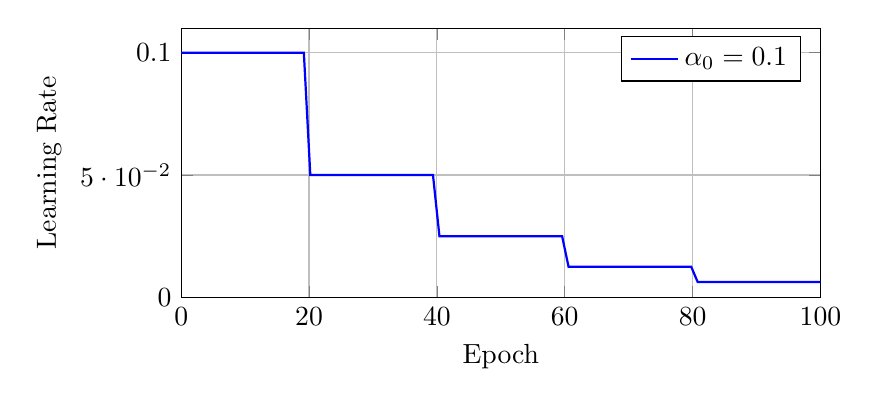
\begin{tikzpicture}
\begin{axis}[
    width=0.8\textwidth,
    height=5cm,
    xlabel={Epoch},
    ylabel={Learning Rate},
    xmin=0, xmax=100,
    ymin=0, ymax=0.11,
    grid=major,
    legend pos=north east,
]
\addplot[blue, thick, samples=100, domain=0:100] {0.1 * 0.5^(floor(x/20))};
\legend{$\alpha_0=0.1$, $\gamma=0.5$, $s=20$}
\end{axis}
\end{tikzpicture}
\end{center}

\textbf{Pros:} Simple, widely used in practice (e.g., every 10 epochs multiply by 0.5)\\
\textbf{Cons:} Requires tuning $\gamma$ and $s$; abrupt changes
\end{frame}

\begin{frame}{Exponential Decay}
\textbf{Formula:}
$$\alpha(t) = \alpha_0 \cdot e^{-\lambda t}$$

where $\lambda > 0$ is the decay rate.

\vspace{0.3cm}

\begin{center}
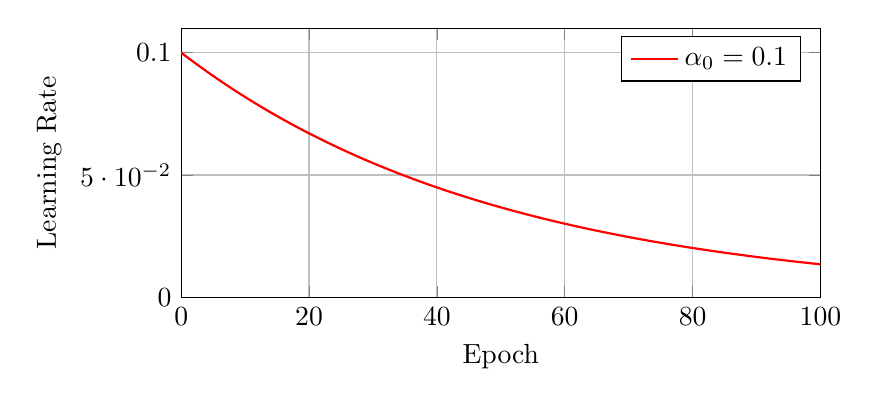
\begin{tikzpicture}
\begin{axis}[
    width=0.8\textwidth,
    height=5cm,
    xlabel={Epoch},
    ylabel={Learning Rate},
    xmin=0, xmax=100,
    ymin=0, ymax=0.11,
    grid=major,
    legend pos=north east,
]
\addplot[red, thick, samples=100, domain=0:100] {0.1 * exp(-0.02*x)};
\legend{$\alpha_0=0.1$, $\lambda=0.02$}
\end{axis}
\end{tikzpicture}
\end{center}

\textbf{Pros:} Smooth decay, theoretically motivated\\
\textbf{Cons:} Can decay too quickly or slowly depending on $\lambda$
\end{frame}

\begin{frame}{1/t Decay (Inverse Time Decay)}
\textbf{Formula:}
$$\alpha(t) = \frac{\alpha_0}{1 + \lambda t}$$

where $\lambda > 0$ controls decay speed.

\vspace{0.3cm}

\begin{center}
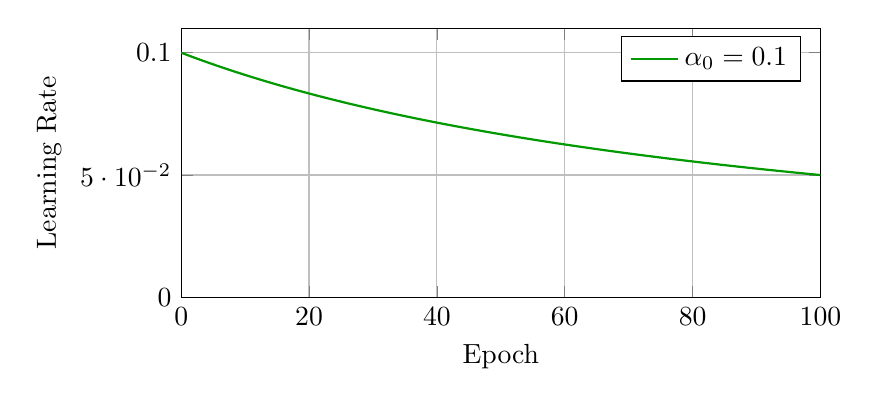
\begin{tikzpicture}
\begin{axis}[
    width=0.8\textwidth,
    height=5cm,
    xlabel={Epoch},
    ylabel={Learning Rate},
    xmin=0, xmax=100,
    ymin=0, ymax=0.11,
    grid=major,
    legend pos=north east,
]
\addplot[green!60!black, thick, samples=100, domain=0:100] {0.1 / (1 + 0.01*x)};
\legend{$\alpha_0=0.1$, $\lambda=0.01$}
\end{axis}
\end{tikzpicture}
\end{center}

\textbf{Pros:} Theoretical guarantees for convex optimization; never reaches zero\\
\textbf{Cons:} Decays slowly initially; may be too aggressive later
\end{frame}

\begin{frame}{Cosine Annealing Schedule}
\textbf{Formula:}
$$\alpha(t) = \alpha_{\min} + \frac{1}{2}(\alpha_0 - \alpha_{\min})\left(1 + \cos\left(\frac{t\pi}{T}\right)\right)$$

where $T$ is the total number of epochs, $\alpha_{\min}$ is minimum learning rate.

\vspace{0.3cm}

\begin{center}
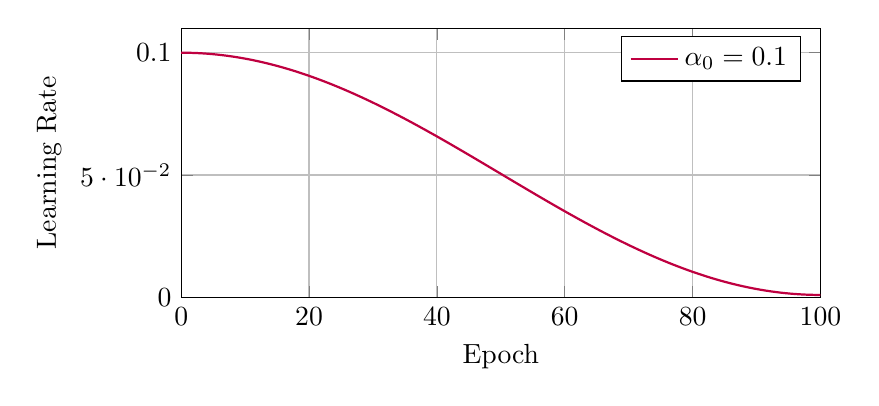
\begin{tikzpicture}
\begin{axis}[
    width=0.8\textwidth,
    height=5cm,
    xlabel={Epoch},
    ylabel={Learning Rate},
    xmin=0, xmax=100,
    ymin=0, ymax=0.11,
    grid=major,
    legend pos=north east,
]
\addplot[purple, thick, samples=200, domain=0:100] {0.001 + 0.5*(0.1 - 0.001)*(1 + cos(deg(x*3.14159/100)))};
\legend{$\alpha_0=0.1$, $\alpha_{\min}=0.001$, $T=100$}
\end{axis}
\end{tikzpicture}
\end{center}

\textbf{Pros:} Smooth decay; popular in deep learning (ResNet training)\\
\textbf{Cons:} Needs to know total epochs in advance
\end{frame}

\begin{frame}{Warmup Schedule}
\textbf{Idea:} Gradually \emph{increase} learning rate at the beginning, then decay.

\vspace{0.2cm}

\textbf{Linear Warmup + Cosine Decay:}
$$\alpha(t) = \begin{cases}
\alpha_0 \cdot \frac{t}{t_{\text{warmup}}} & \text{if } t \leq t_{\text{warmup}} \\
\alpha_{\min} + \frac{1}{2}(\alpha_0 - \alpha_{\min})\left(1 + \cos\left(\frac{(t-t_{\text{warmup}})\pi}{T-t_{\text{warmup}}}\right)\right) & \text{otherwise}
\end{cases}$$

\begin{center}
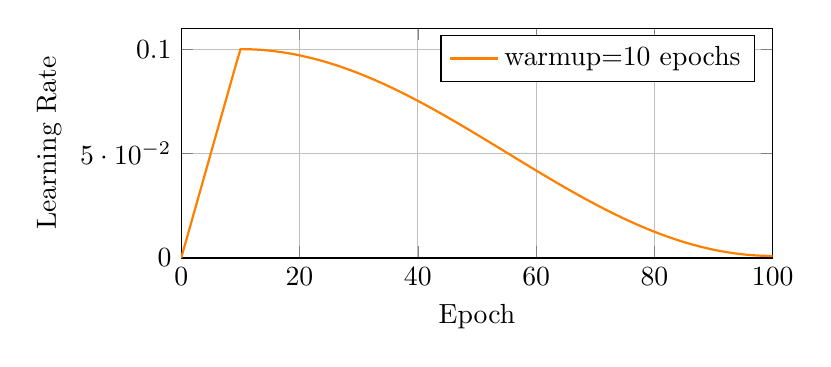
\begin{tikzpicture}
\begin{axis}[
    width=0.75\textwidth,
    height=4.5cm,
    xlabel={Epoch},
    ylabel={Learning Rate},
    xmin=0, xmax=100,
    ymin=0, ymax=0.11,
    grid=major,
    legend pos=north east,
]
\addplot[orange, thick, samples=200, domain=0:100] {
    (x <= 10) ? (0.1 * x / 10) : 
    (0.001 + 0.5*(0.1 - 0.001)*(1 + cos(deg((x-10)*3.14159/(100-10)))))
};
\legend{warmup=10 epochs}
\end{axis}
\end{tikzpicture}
\end{center}

\textbf{Motivation:} Prevents instability with large batch sizes; used in Transformers (BERT, GPT)
\end{frame}

\begin{frame}{Comparison of Schedules}
\begin{center}
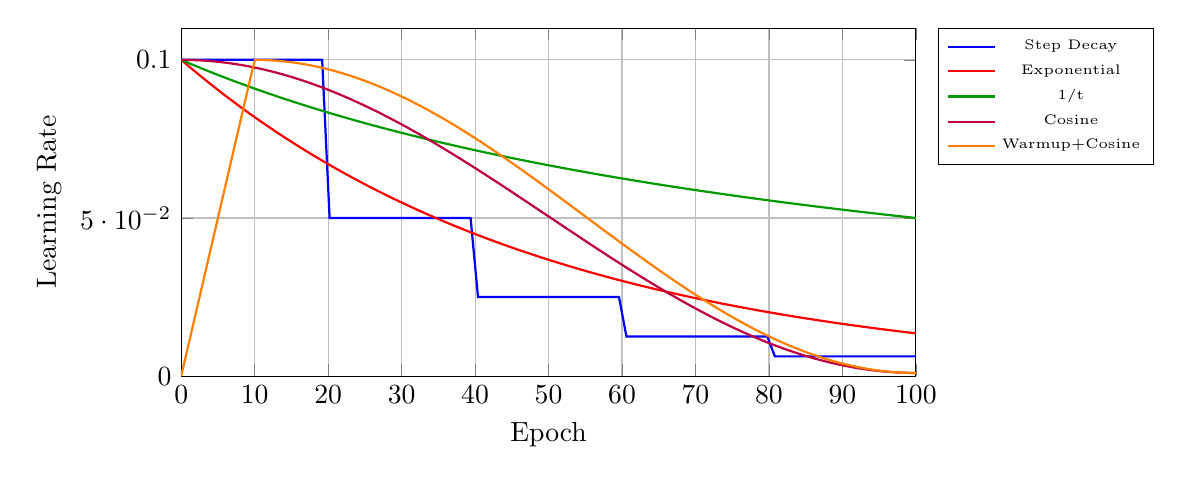
\begin{tikzpicture}
\begin{axis}[
    width=0.9\textwidth,
    height=6cm,
    xlabel={Epoch},
    ylabel={Learning Rate},
    xmin=0, xmax=100,
    ymin=0, ymax=0.11,
    grid=major,
    legend pos=outer north east,
    legend style={font=\tiny},
]
% Step decay
\addplot[blue, thick, samples=100, domain=0:100] {0.1 * 0.5^(floor(x/20))};
% Exponential
\addplot[red, thick, samples=100, domain=0:100] {0.1 * exp(-0.02*x)};
% 1/t
\addplot[green!60!black, thick, samples=100, domain=0:100] {0.1 / (1 + 0.01*x)};
% Cosine
\addplot[purple, thick, samples=200, domain=0:100] {0.001 + 0.5*(0.1 - 0.001)*(1 + cos(deg(x*3.14159/100)))};
% Warmup
\addplot[orange, thick, samples=200, domain=0:100] {
    (x <= 10) ? (0.1 * x / 10) : 
    (0.001 + 0.5*(0.1 - 0.001)*(1 + cos(deg((x-10)*3.14159/(100-10)))))
};
\legend{Step Decay, Exponential, 1/t, Cosine, Warmup+Cosine}
\end{axis}
\end{tikzpicture}
\end{center}
\end{frame}



\begin{frame}
	\centering
	\Huge GD Weaknesses

\end{frame}

\section{Weakness - Ill Conditioning}



\includepdf[pages={33-40}, scale=1.35, offset=2.5cm -0.5cm]{slides_lmu/04_first_order.pdf}

\section{Weakness - Saddle Points and Multimodality}

\includepdf[pages={43-56}, scale=1.35, offset=2.5cm -0.5cm]{slides_lmu/04_first_order.pdf}

\end{document}